\documentclass{fkssolpub}

\usepackage[czech]{babel}
\usepackage{fontspec}
\usepackage{fkssugar}
\usepackage{amsmath}
\usepackage{graphicx}

\author{Ondřej Sedláček}
\school{Gymnázium Oty Pavla} 
\series{FO-B-S}
\problem{5} 

\begin{document} 

V části \textit{a} nám fakt, že se teplota ustálila, říká, že už žádný
výkon vařiče se nepoužívá na přidání tepla vodě, ale že už všechno teplo
uniká do okolí. Tím pádem platí:

\[
  P_{01} = \beta (t_h - t_o)
\]

z čehož již jednoduše konstantu přenosu odvodíme:

\[
  \beta = \frac{P_{01}}{t_h - t_o} = 10 \text{J} \cdot \text{s}^{-1} \cdot \text{K}^{-1}
\]

Nejmenší výkon vařiče pro zahřátí vody na teplotu varu určíme díky již
známé konstantě $\beta$ snadno. V bodě varu musí docházet k úniku veškerého
výkonu, proto:

\[
  P_{0min} = \beta (t_h - t_o) = 800 \text{W}
\]

Graf závislosti maximální teploty na výkonu je níže:

\begin{figure}[h!]
  \centering
  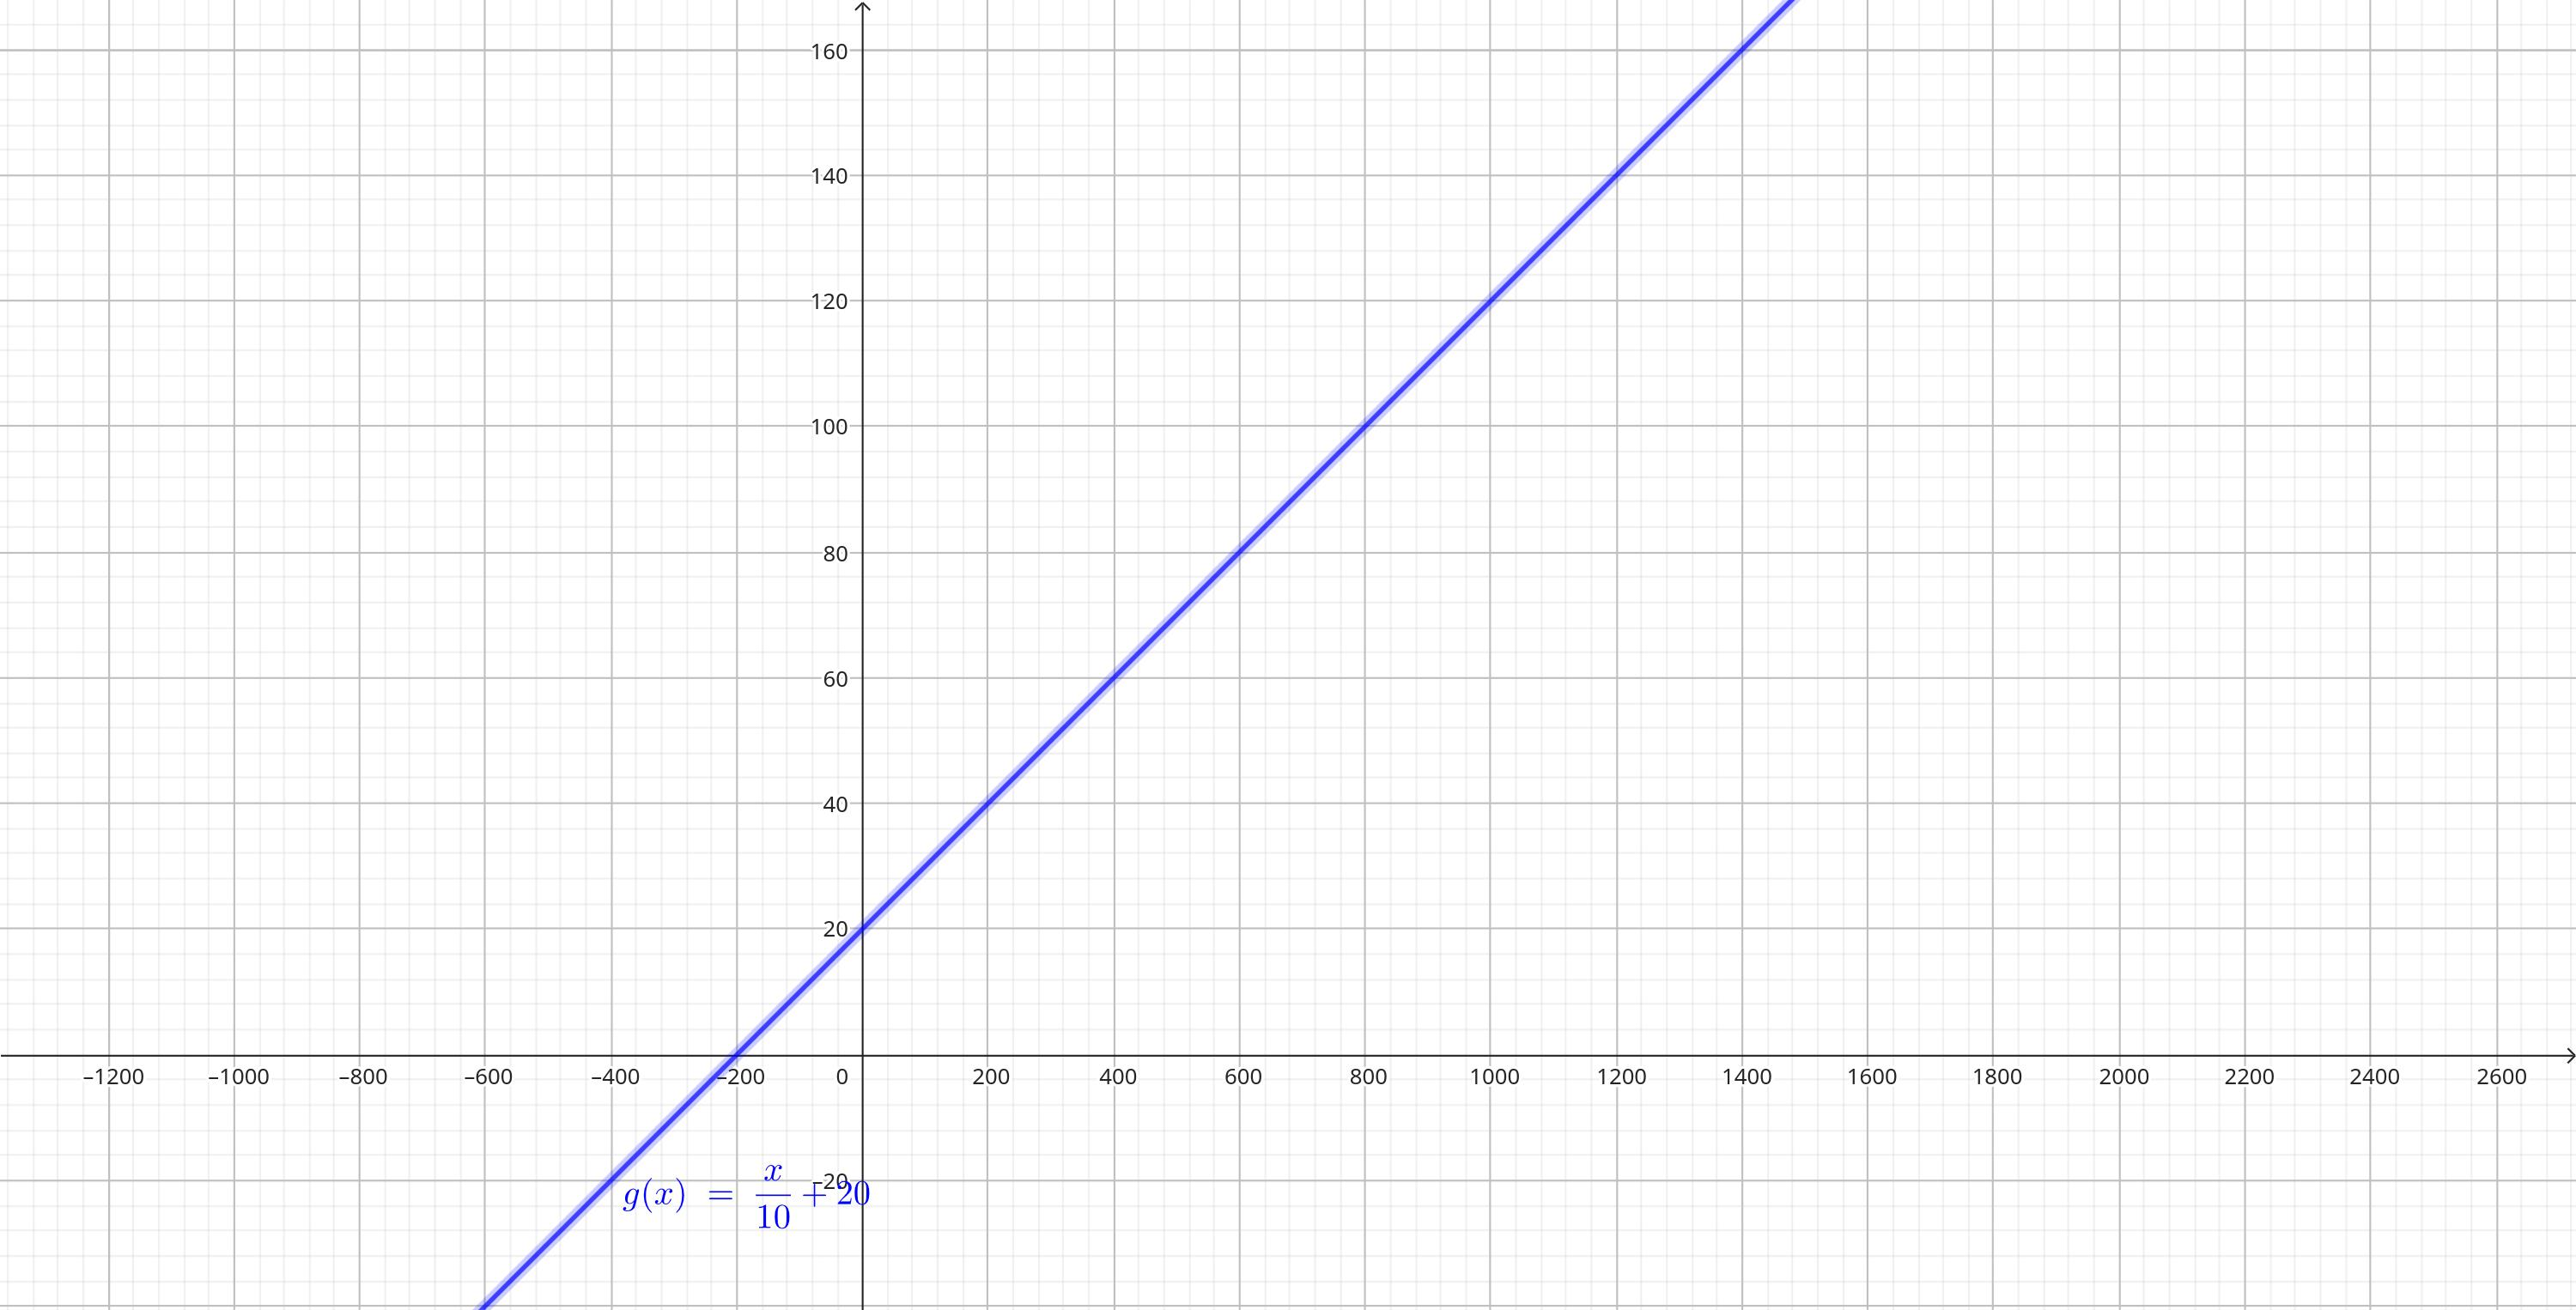
\includegraphics[width=0.95\textwidth]{5-fig.jpg}
  \caption{Graf závislosti maximální teploty (v $^{\circ}$C) na výkonu}
  \label{fig:1}
\end{figure}

V části \textit{d} zjistíme rychlost změny teploty tak, že zjistíme výkon
použitý pro ohřev a následně vypočítáme změnu teploty za jednu sekundu
přes kalorimetrickou rovnici:

\[
  P_{0max} - \beta (20 - 20) = C \Delta t
\]
\[
  v_p = \frac{P_{0max}}{C} = \frac{1}{3} \text{K} \cdot \text{s}^{-1}
\]

Podobně zjistíme rychlost ohřevu v bodě varu:

\[
  P_{0max} - \beta (100 - 20) = C \Delta t
\]
\[
  v_v = \frac{P_{0max} - 80 \beta}{C} = \frac{7}{45} \text{K} \cdot \text{s}^{-1}
\]

Pro část \textit{e} nejprve vyřešíme rovnici:

\[
  \frac{v_p + v_v}{2} t = 100 - 20
\]
\[
  t = \frac{160}{v_p + v_v} = \frac{3600}{11} \text{s}
\]

Uniklé teplo pak vypočítáme jako rozdíl tepla dodané vařičem a teplo uložené
v hrnci s vodou:

\[
  \frac{Q_u}{Q_d} = 1 - \frac{(100 - 20) C}{P_{0max} t} = \frac{4}{15} \doteq 27 \%
\]

\end{document}
